\begin{frame}
	\frametitle{Modelos Lineares para a Procura: Exemplo}
	{\color{blue} Procura \textbf{individual} de p\~ao sem gl\'uten}

	\vspace{0.2cm}
	
	\begin{columns}
		\begin{column}{0.28\textwidth}
			{\color{red}Quadro:}\vspace{0.2cm}
			\begin{tabular}{|c|c|}
				\hline
				Pre\c co & Quantidade \\
				\hline
				0 & 50 \\
				1 & 40 \\
				2 & 30 \\
				3 & 20 \\
				4 & 10 \\
				5 & 0 \\ \hline
			\end{tabular}
			\only<4>{
				Declive da reta?
				\[\frac{d p}{d Q}=\frac{\Delta p}{\Delta Q}=-0.1\]
			}
		\end{column}
		\begin{column}{0.68\textwidth}
		\begin{tabular}{rc}
			{\color{red}Equa\c c\~ao:}& \(Q^D = 50 - 10\times P\)  \\
								ou	  &	\(P = 5 - \frac{1}{10}Q^D\)\\
			{\color{red}Gr\'afico:}	&
		\end{tabular}
		
		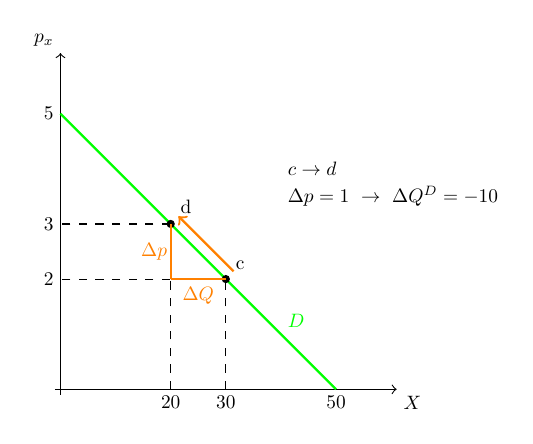
\begin{tikzpicture}[
			scale = 0.7,
			every node/.style = {scale=0.7},
			declare function = {d(\x)=5-\x;}
			]

			\draw[->] (-0.1,0) -- (6.1,0)node[below right] {$X$};
			\draw[->] (0,-0.1) -- (0,6.1)node[above left] {$p_x$};

			\draw[domain=0:5,variable=\x,green,thick] plot (\x,{d(\x)});
			\draw(4,{d(4)}) node[green,above right]{$D$};
			\draw(0,{d(0)}) node[left]{5};
			\draw(5,0) node[below]{50};

			\onslide<2-3>{
				\draw[dashed](3,0) node[below]{30} -- (3,{d(3)})node[circle,fill,inner sep=1.5pt,label=above right:c]{} -- (0,{d(3)}) node[left]{2};
				\draw[dashed](2,0) node[below]{20} -- (2,{d(2)})node[circle,fill,inner sep=1.5pt,label=above right:d]{} -- (0,{d(2)}) node[left]{3};
				\draw(4,4) node[right]{\(c\rightarrow d\)};
			}

			\onslide<3-4>{
				\draw[->,thick,orange] (3+0.14,{d(3)+0.14}) -- (2+0.14,{d(2)+0.14});
				\draw(4,3.5) node[right]{\(\Delta p = 1 \ \rightarrow\ \Delta Q^D=-10\)};
				\draw[thick,orange](2,{d(3)})--(3,{d(3)})node[midway,yshift=-0.3cm]{$\Delta Q$};
				\draw[thick,orange](2,{d(2)})--(2,{d(3)})node[midway,xshift=-0.3cm]{$\Delta p$};
			}

		\end{tikzpicture}
		\end{column}
	\end{columns}
\end{frame}

\begin{frame}
	\frametitle{Modelos Lineares para a procura: Exemplo}
	{\color{blue} Procura \textbf{de mercado} de p\~ao sem gl\'uten: N=2}

	\vspace{0.2cm}
	
	\begin{columns}

		\begin{column}{0.25\textwidth}
		{\footnotesize
		{\color{green}Consumidor 1}\\
		\(Q_1^D=50-10\times p\)
		\(P=5-0.1\times Q\)
		}
		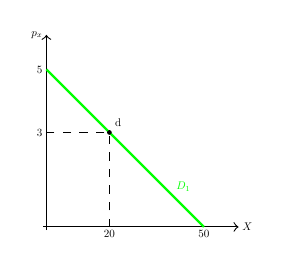
\begin{tikzpicture}[
			scale = 0.4,
			every node/.style = {scale=0.4},
			declare function = {d(\x)=5-\x;}
			]

			\draw[->] (-0.1,0) -- (6.1,0)node[right] {$X$};
			\draw[->] (0,-0.1) -- (0,6.1)node[left] {$p_x$};

			\draw[domain=0:5,variable=\x,green,thick] plot (\x,{d(\x)});
			\draw(4,{d(4)}) node[green,above right]{$D_1$};
			\draw(0,{d(0)}) node[left]{5};
			\draw(5,0) node[below]{50};

			\draw[dashed](2,0) node[below]{20} -- (2,{d(2)})node[circle,fill,inner sep=1.5pt,label=above right:d]{} -- (0,{d(2)}) node[left]{3};

		\end{tikzpicture}
		\end{column}
		
		\begin{column}{0.25\textwidth}
		{\footnotesize
		{\color{red}Consumidor 2}\\
		\(Q_2^D=50-10\times p\)
		\(P=5-0.1\times Q\)
		}
		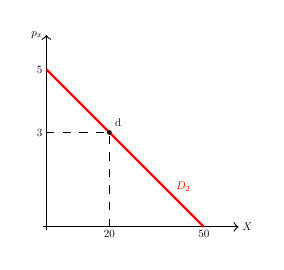
\begin{tikzpicture}[
			scale = 0.4,
			every node/.style = {scale=0.4},
			declare function = {d(\x)=5-\x;}
			]

			\draw[->] (-0.1,0) -- (6.1,0)node[right] {$X$};
			\draw[->] (0,-0.1) -- (0,6.1)node[left] {$p_x$};

			\draw[domain=0:5,variable=\x,red,thick] plot (\x,{d(\x)});
			\draw(4,{d(4)}) node[red,above right]{$D_2$};
			\draw(0,{d(0)}) node[left]{5};
			\draw(5,0) node[below]{50};

			\draw[dashed](2,0) node[below]{20} -- (2,{d(2)})node[circle,fill,inner sep=1.5pt,label=above right:d]{} -- (0,{d(2)}) node[left]{3};

		\end{tikzpicture}
		\end{column}
		\begin{column}{0.5\textwidth}
		{\footnotesize
		{\color{blue}Mercado}\\
		\(Q_M^D=100-20\times p\)\\
		\(P=5-0.05\times Q\)
		}
		\begin{tikzpicture}[
			scale = 0.4,
			every node/.style = {scale=0.4},
			declare function = {d(\x)=5-0.5*\x;}
			]

			\draw[->] (-0.1,0) -- (11.1,0)node[right] {$X$};
			\draw[->] (0,-0.1) -- (0,6.1)node[left] {$p_x$};

			\draw[domain=0:10,variable=\x,blue,thick] plot (\x,{d(\x)});
			\draw(8,{d(8)}) node[blue,above right]{$D_{mercado}$};
			\draw(0,{d(0)}) node[left]{5};
			\draw(10,0) node[below]{100};

			\draw[dashed](4,0) node[below]{40} -- (4,{d(4)})node[circle,fill,inner sep=1.5pt,label=above right:d]{} -- (0,{d(4)}) node[left]{3};

		\end{tikzpicture}
		\end{column}
	\end{columns}
	\vspace{0.4cm}
	A agrega\c c\~ao \'e sempre horizontal: O que se adiciona s\~ao quantidades, n\~ao pre\c cos. Se juntamos dois consumidores iguais, n\~ao \'e a mesma quantidade ao dobro do pre\c co, mas sim o dobro da quantidade ao mesmo pre\c co!!!
\end{frame}


\begin{frame}
	\frametitle{Curva de Procura Individual e altera\c c\~oes de rendimento}
	\begin{center}
			\def\rho{0.5}
			\def\ww{10}
			\def\whw{22}
			\def\pyy{3}
			\def\pxx{3}
			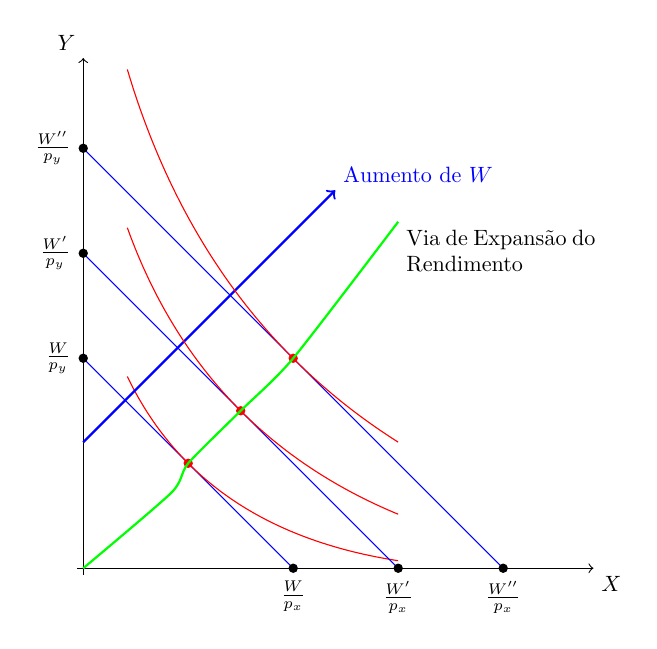
\begin{tikzpicture}[
				scale = 0.8,
				every node/.style={scale = 0.8},
				declare function={
					x(\w,\px,\py) = (\w*(\px^(1/(\rho-1))))/(\px^(\rho/(\rho-1))+\py^(\rho/(\rho-1)));
					y(\w,\px,\py) = (\w*(\py^(1/(\rho-1))))/(\px^(\rho/(\rho-1))+\py^(\rho/(\rho-1)));
					u(\x,\y) = (\x^\rho+\y^\rho)^(1/\rho);
					ic(\w,\x,\px,\py) = (u(x(\w,\px,\py),y(\w,\px,\py))^\rho-\x^\rho)^(1/\rho);
					bc(\w,\x,\px,\py) = \w/\py - (\px/\py)*\x;
				}
				]

				\draw[->] (-0.1,0) -- (8.1,0)node[below right] {$X$};
				\draw[->] (0,-0.1) -- (0,8.1)node[above left] {$Y$};

				\draw[samples=100,blue,domain=0:(10/\pxx),variable=\x] plot (\x,{bc(10,\x,\pxx,\pyy)});
				\draw({10/\pxx},0) node[circle,fill,inner sep=1.5pt,label=below :\(\frac{W}{p_x}\)]{};
				\draw(0,{10/\pyy}) node[circle,fill,inner sep=1.5pt,label=left :\(\frac{W}{p_y}\)]{};
				\draw[samples=100,red,domain=.70:5,variable=\x] plot (\x,{ic(10,\x,\pxx,\pyy)});
				\draw({x(10,\pxx,\pyy)},{y(10,\pxx,\pyy)}) node[red,circle,fill,inner sep=1.5pt]{};

				\onslide<2->{
					\draw[->,blue,thick] (0,2) -- (4,6) node[above right]{\parbox[l]{3cm}{Aumento de $W$}};
					\draw[samples=100,blue,domain=0:(15/\pxx),variable=\x] plot (\x,{bc(15,\x,\pxx,\pyy)});
					\draw({15/\pxx},0) node[circle,fill,inner sep=1.5pt,label=below :\(\frac{W'}{p_x}\)]{};
					\draw(0,{15/\pyy}) node[circle,fill,inner sep=1.5pt,label=left :\(\frac{W'}{p_y}\)]{};
					\draw[samples=100,red,domain=.70:5,variable=\x] plot (\x,{ic(15,\x,\pxx,\pyy)});
					\draw({x(15,\pxx,\pyy)},{y(15,\pxx,\pyy)}) node[red,circle,fill,inner sep=1.5pt]{};				
				}

				\onslide<3->{
					\draw[samples=100,blue,domain=0:(20/\pxx),variable=\x] plot (\x,{bc(20,\x,\pxx,\pyy)});
					\draw({20/\pxx},0) node[circle,fill,inner sep=1.5pt,label=below :\(\frac{W''}{p_x}\)]{};
					\draw(0,{20/\pyy}) node[circle,fill,inner sep=1.5pt,label=left :\(\frac{W''}{p_y}\)]{};
					\draw[samples=100,red,domain=.70:5,variable=\x] plot (\x,{ic(20,\x,\pxx,\pyy)});
					\draw({x(20,\pxx,\pyy)},{y(20,\pxx,\pyy)}) node[red,circle,fill,inner sep=1.5pt]{};				
				}

				\onslide<4->{
					\draw[thick,green] plot[smooth,tension=0.4] coordinates{(0,0) (1.4,1.2) ({x(10,\pxx,\pyy)},{y(10,\pxx,\pyy)}) ({x(15,\pxx,\pyy)},{y(15,\pxx,\pyy)}) ({x(20,\pxx,\pyy)},{y(20,\pxx,\pyy)}) (5,5.5)} node[black,below right]{\parbox[l]{3cm}{Via de Expans\~ao do Rendimento}};
				}

			\end{tikzpicture}
		\end{center}
\end{frame}

\begin{frame}
	\frametitle{Via de Expans\~ao de Rendimento e Curvas de Engel (bens normais)}
		\begin{center}
			\def\rho{0.5}
			\def\pyy{3}
			\def\pxx{3}
			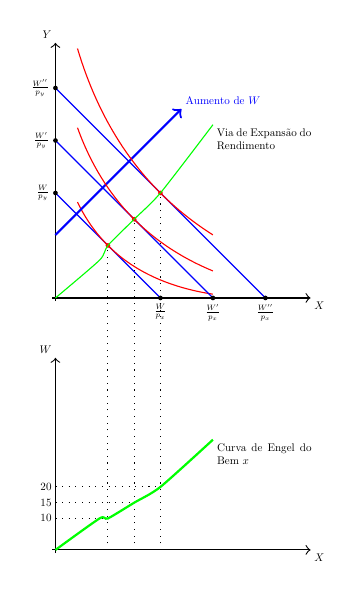
\begin{tikzpicture}[
				scale = 0.4,
				every node/.style={scale = 0.4},
				declare function={
					x(\w,\px,\py) = (\w*(\px^(1/(\rho-1))))/(\px^(\rho/(\rho-1))+\py^(\rho/(\rho-1)));
					y(\w,\px,\py) = (\w*(\py^(1/(\rho-1))))/(\px^(\rho/(\rho-1))+\py^(\rho/(\rho-1)));
					u(\x,\y) = (\x^\rho+\y^\rho)^(1/\rho);
					ic(\w,\x,\px,\py) = (u(x(\w,\px,\py),y(\w,\px,\py))^\rho-\x^\rho)^(1/\rho);
					bc(\w,\x,\px,\py) = \w/\py - (\px/\py)*\x;
				}
				]

				\draw[->] (-0.1,0) -- (8.1,0)node[below right] {$X$};
				\draw[->] (0,-0.1) -- (0,8.1)node[above left] {$Y$};

				\draw[samples=100,blue,domain=0:(10/\pxx),variable=\x] plot (\x,{bc(10,\x,\pxx,\pyy)});
				\draw({10/\pxx},0) node[circle,fill,inner sep=1.5pt,label=below :\(\frac{W}{p_x}\)]{};
				\draw(0,{10/\pyy}) node[circle,fill,inner sep=1.5pt,label=left :\(\frac{W}{p_y}\)]{};
				\draw[samples=100,red,domain=.70:5,variable=\x] plot (\x,{ic(10,\x,\pxx,\pyy)});
				\draw({x(10,\pxx,\pyy)},{y(10,\pxx,\pyy)}) node[red,circle,fill,inner sep=1.5pt]{};

				\draw[->,blue,thick] (0,2) -- (4,6) node[above right]{\parbox[l]{3cm}{Aumento de $W$}};
				\draw[samples=100,blue,domain=0:(15/\pxx),variable=\x] plot (\x,{bc(15,\x,\pxx,\pyy)});
				\draw({15/\pxx},0) node[circle,fill,inner sep=1.5pt,label=below :\(\frac{W'}{p_x}\)]{};
				\draw(0,{15/\pyy}) node[circle,fill,inner sep=1.5pt,label=left :\(\frac{W'}{p_y}\)]{};
				\draw[samples=100,red,domain=.70:5,variable=\x] plot (\x,{ic(15,\x,\pxx,\pyy)});
				\draw({x(15,\pxx,\pyy)},{y(15,\pxx,\pyy)}) node[red,circle,fill,inner sep=1.5pt]{};				

				\draw[samples=100,blue,domain=0:(20/\pxx),variable=\x] plot (\x,{bc(20,\x,\pxx,\pyy)});
				\draw({20/\pxx},0) node[circle,fill,inner sep=1.5pt,label=below :\(\frac{W''}{p_x}\)]{};
				\draw(0,{20/\pyy}) node[circle,fill,inner sep=1.5pt,label=left :\(\frac{W''}{p_y}\)]{};
				\draw[samples=100,red,domain=.70:5,variable=\x] plot (\x,{ic(20,\x,\pxx,\pyy)});
				\draw({x(20,\pxx,\pyy)},{y(20,\pxx,\pyy)}) node[red,circle,fill,inner sep=1.5pt]{};				

				\draw[green] plot[smooth,tension=0.4] coordinates{(0,0) (1.4,1.2) ({x(10,\pxx,\pyy)},{y(10,\pxx,\pyy)}) ({x(15,\pxx,\pyy)},{y(15,\pxx,\pyy)}) ({x(20,\pxx,\pyy)},{y(20,\pxx,\pyy)}) (5,5.5)} node[black,below right]{\parbox[l]{3cm}{Via de Expans\~ao do Rendimento}};

				\draw[->] (-0.1,-8) -- (8.1,-8)node[below right] {$X$};
				\draw[->] (0,-8.1) -- (0,-1.9)node[above left] {$W$};

				\onslide<3->{
					\draw[dotted] (0,{1-8}) node[left]{10} -- ({x(10,\pxx,\pyy)},{1-8});
					\draw[dotted] (0,{1.5-8}) node[left]{15} -- ({x(15,\pxx,\pyy)},{1.5-8});
					\draw[dotted] (0,{2-8}) node[left]{20} -- ({x(20,\pxx,\pyy)},{2-8});
				}

				\onslide<2->{
					\draw[dotted] ({x(10,\pxx,\pyy)},-8) -- ({x(10,\pxx,\pyy)},{y(10,\pxx,\pyy)});
					\draw[dotted] ({x(15,\pxx,\pyy)},-8) -- ({x(15,\pxx,\pyy)},{y(15,\pxx,\pyy)});
					\draw[dotted] ({x(20,\pxx,\pyy)},-8) -- ({x(20,\pxx,\pyy)},{y(20,\pxx,\pyy)});	
				}

				\onslide<4->{
					\draw[thick,green] plot[smooth,tension=0.4] coordinates{
						(0,-8)
						(1.4,{1.0-8})
						({x(10,\pxx,\pyy)},{1-8})
						({x(15,\pxx,\pyy)},{1.5-8})
						({x(20,\pxx,\pyy)},{2.0-8})
						(5,{3.5-8})
						} node[black,below right]{\parbox[l]{3cm}{Curva de Engel do Bem \(x\)}};
				}

			\end{tikzpicture}
		\end{center}
\end{frame}

\begin{frame}
	\frametitle{Caso o bem $X$ seja um bem inferior}
		\begin{center}
			\def\rho{0.5}
			\def\pyy{3}
			\def\pxx{3}
			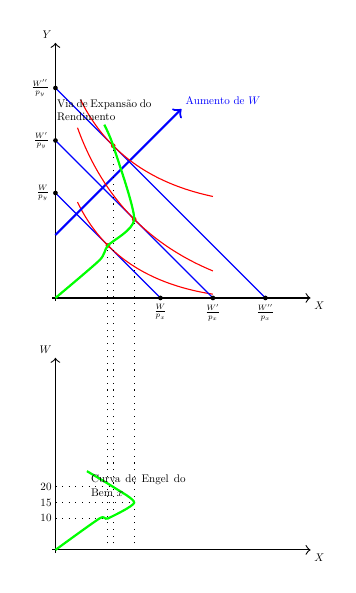
\begin{tikzpicture}[
				scale = 0.4,
				every node/.style={scale = 0.4},
				declare function={
					x(\w,\px,\py) = (\w*(\px^(1/(\rho-1))))/(\px^(\rho/(\rho-1))+\py^(\rho/(\rho-1)));
					y(\w,\px,\py) = (\w*(\py^(1/(\rho-1))))/(\px^(\rho/(\rho-1))+\py^(\rho/(\rho-1)));
					u(\x,\y) = (\x^\rho+\y^\rho)^(1/\rho);
					ic(\w,\x,\px,\py) = (u(x(\w,\px,\py),y(\w,\px,\py))^\rho-\x^\rho)^(1/\rho);
					ic2(\w,\x,\px,\py) = (u(x(\w,\px,\py),y(\w,\px,\py))^\rho-\x^\rho)^(1/\rho)+3;
					bc(\w,\x,\px,\py) = \w/\py - (\px/\py)*\x;
				}
				]

				\draw[->] (-0.1,0) -- (8.1,0)node[below right] {$X$};
				\draw[->] (0,-0.1) -- (0,8.1)node[above left] {$Y$};

				\draw[samples=100,blue,domain=0:(10/\pxx),variable=\x] plot (\x,{bc(10,\x,\pxx,\pyy)});
				\draw({10/\pxx},0) node[circle,fill,inner sep=1.5pt,label=below :\(\frac{W}{p_x}\)]{};
				\draw(0,{10/\pyy}) node[circle,fill,inner sep=1.5pt,label=left :\(\frac{W}{p_y}\)]{};
				\draw[samples=100,red,domain=.70:5,variable=\x] plot (\x,{ic(10,\x,\pxx,\pyy)});
				\draw({x(10,\pxx,\pyy)},{y(10,\pxx,\pyy)}) node[red,circle,fill,inner sep=1.5pt]{};

				\draw[->,blue,thick] (0,2) -- (4,6) node[above right]{\parbox[l]{3cm}{Aumento de $W$}};
				\draw[samples=100,blue,domain=0:(15/\pxx),variable=\x] plot (\x,{bc(15,\x,\pxx,\pyy)});
				\draw({15/\pxx},0) node[circle,fill,inner sep=1.5pt,label=below :\(\frac{W'}{p_x}\)]{};
				\draw(0,{15/\pyy}) node[circle,fill,inner sep=1.5pt,label=left :\(\frac{W'}{p_y}\)]{};
				\draw[samples=100,red,domain=.70:5,variable=\x] plot (\x,{ic(15,\x,\pxx,\pyy)});
				\draw({x(15,\pxx,\pyy)},{y(15,\pxx,\pyy)}) node[red,circle,fill,inner sep=1.5pt]{};				

				\draw[samples=100,blue,domain=0:(20/\pxx),variable=\x] plot (\x,{bc(20,\x,\pxx,\pyy)});
				\draw({20/\pxx},0) node[circle,fill,inner sep=1.5pt,label=below :\(\frac{W''}{p_x}\)]{};
				\draw(0,{20/\pyy}) node[circle,fill,inner sep=1.5pt,label=left :\(\frac{W''}{p_y}\)]{};
				\draw[samples=100,red,domain=.80:5,variable=\x] plot (\x,{ic2(11,\x,\pxx,\pyy)});
				\draw({x(11,\pxx,\pyy)},{ic2(11,x(11,\pxx,\pyy),\pxx,\pyy)}) node[red,circle,fill,inner sep=1.5pt]{};				

				\draw[thick,green] plot[smooth,tension=0.4] coordinates{
					(0,0)
					(1.4,1.2)
					({x(10,\pxx,\pyy)},{y(10,\pxx,\pyy)})
					({x(15,\pxx,\pyy)},{y(15,\pxx,\pyy)})
					({x(11,\pxx,\pyy)},{ic2(11,x(11,\pxx,\pyy),\pxx,\pyy)})
					(1.55,5.5)
				} node[black,above]{\parbox[l]{3cm}{Via de Expans\~ao do Rendimento}};

				\draw[->] (-0.1,-8) -- (8.1,-8)node[below right] {$X$};
				\draw[->] (0,-8.1) -- (0,-1.9)node[above left] {$W$};

				\draw[dotted] (0,{1-8}) node[left]{10} -- ({x(10,\pxx,\pyy)},{1-8});
				\draw[dotted] (0,{1.5-8}) node[left]{15} -- ({x(15,\pxx,\pyy)},{1.5-8});
				\draw[dotted] (0,{2-8}) node[left]{20} -- ({x(11,\pxx,\pyy)},{2-8});

				\draw[dotted] ({x(10,\pxx,\pyy)},-8) -- ({x(10,\pxx,\pyy)},{y(10,\pxx,\pyy)});
				\draw[dotted] ({x(15,\pxx,\pyy)},-8) -- ({x(15,\pxx,\pyy)},{y(15,\pxx,\pyy)});
				\draw[dotted] ({x(11,\pxx,\pyy)},-8) -- ({x(11,\pxx,\pyy)},{ic2(11,x(11,\pxx,\pyy),\pxx,\pyy)});	

				\draw[thick,green] plot[smooth,tension=0.4] coordinates{
						(0,-8)
						(1.4,{1.0-8})
						({x(10,\pxx,\pyy)},{1-8})
						({x(15,\pxx,\pyy)},{1.5-8})
						({x(11,\pxx,\pyy)},{2.0-8})
						(1,{2.5-8})
					} node[black,below right]{\parbox[l]{3cm}{Curva de Engel do Bem \(x\)}};

			\end{tikzpicture}
		\end{center}
\end{frame}


% \begin{frame}
% 	\frametitle{Lei da Procura}
% 	Voltemos \`a rela\c c\~ao negativa entre quantidade procurada de um bem e pre\c co desse mesmo bem!

% 	\vspace{0.5cm}

% 	A rela\c c\~ao fiocu demonstrada graficamente, mas quais as raz\~oes efectivas para esta conclus\~ao?

% 	\vspace{0.4cm}

% 	Vejamos...
% \end{frame}

% \begin{frame}
% 	\frametitle{Lei da Procura}
% 	\begin{center}
% 	\LARGE A altera\c c\~ao no pre\c co do bem leva a uma altera\c c\~ao do seu consumo devido a dois efeitos:
% 	\end{center}
% \end{frame}

% \begin{frame}
% 	\frametitle{Efeito Substitui\c c\~ao e Efeito Rendimento ap\'os $\Delta p$}

% 	\textbf{\underline{Efeito substitui\c c\~ao:}} se o pre\c co de um bem aumenta (\emph{c\ae teris paribus}), a quantidade procurada diminui porque os consumidores olham para alternativas que satisfa\c cam a mesma necessidade, passando alguns deles a adquirir esses bens substitutos
% \end{frame}

% \begin{frame}
% 	\frametitle{Efeito Substitui\c c\~ao e Efeito Rendimento ap\'os $\Delta p$}
% 	\textbf{\underline{Efeito rendimento:}} se o pre\c co de um bem aumenta (\emph{c\ae teris paribus}), a quantidade procurada diminui porque os consumidores se sentem mais pobres com o \textbf{\underline{mesmo rendimento}} e reduzem o seu consumo (quebra de poder de compra)

% 	\vspace{1cm}

% 	Nota: Efeito rendimento $\neq$ Altera\c c\~oes no rendimento
% \end{frame}

% \begin{frame}
% 	\frametitle{Efeitos substitui\c c\~ao (Hicks) e Rendimento (x bem normal)}
% 	\begin{center}
% 			\def\rho{0.5}
% 			\def\pxx{3}
% 			\def\pyy{3}
% 			\def\qxx{5}
% 			\def\qyy{4}
% 			\begin{tikzpicture}[
% 				scale = 0.7,
% 				every node/.style={scale = 0.7},
% 				declare function={
% 					x(\w,\px,\py) = (\w*(\px^(1/(\rho-1))))/(\px^(\rho/(\rho-1))+\py^(\rho/(\rho-1)));
% 					y(\w,\px,\py) = (\w*(\py^(1/(\rho-1))))/(\px^(\rho/(\rho-1))+\py^(\rho/(\rho-1)));
% 					u(\x,\y) = (\x^\rho+\y^\rho)^(1/\rho);
% 					ic(\w,\x,\px,\py) = (u(x(\w,\px,\py),y(\w,\px,\py))^\rho-\x^\rho)^(1/\rho);
% 					bc(\w,\x,\px,\py) = \w/\py - (\px/\py)*\x;
% 				}
% 				]

% 				\draw[->] (-0.1,0) -- (8.1,0)node[below right] {$X$};
% 				\draw[->] (0,-0.1) -- (0,8.1)node[above left] {$Y$};

% 				\draw[samples=100,blue,domain=0:(20/\pxx),variable=\x] plot (\x,{bc(20,\x,\pxx,\pyy)});
% 				\draw({20/\pxx},0) node[circle,fill,inner sep=1.5pt,label=below :\(\frac{W}{p_x}\)]{};
% 				\draw(0,{20/\pyy}) node[circle,fill,inner sep=1.5pt,label=left :\(\frac{W}{p_y}\)]{};
% 				\draw[samples=100,red,domain=.9:6,variable=\x] plot (\x,{ic(20,\x,\pxx,\pyy)});
% 				\draw({x(20,\pxx,\pyy)},{y(20,\pxx,\pyy)}) node[red,circle,fill,inner sep=1.5pt,label=above right:{\(A^*(P,W)\)}]{};
				
% 				\onslide<2->{
% 					\draw[samples=100,blue,domain=0:(20/\qxx),variable=\x] plot (\x,{bc(20,\x,\qxx,\pyy)});
% 					\draw({20/\qxx},0) node[circle,fill,inner sep=1.5pt,label=below :\(\frac{W}{p_x'}\)]{};
% 					\draw(0,{20/\pyy}) node[circle,fill,inner sep=1.5pt,label=left :\(\frac{W}{p_y}\)]{};
% 					\draw[samples=100,red,domain=.65:5,variable=\x] plot (\x,{ic(20,\x,\qxx,\pyy)});
% 					\draw({x(20,\qxx,\pyy)},{y(20,\qxx,\pyy)}) node[red,circle,fill,inner sep=1.5pt,label=below left:{\(A^*(P',W)\)}]{};
% 				}

% 				\onslide<3->{
% 					\draw[samples=100,green,thick,domain=0:(20/\qxx),variable=\x] plot (\x,{bc(25,\x,\qxx,\pyy)});
% 					\draw(2,5) node[red,circle,fill,inner sep=1.5pt,label=above right:{\(A^s\)}]{};
% 				}

% 				\onslide<4->{
% 					\draw[->,thick] ({x(20,\pxx,\pyy)},{y(20,\pxx,\pyy)}) -- (2,{y(20,\pxx,\pyy)}) node[below right]{Efeito Substitui\c c\~ao};
% 					\draw[dotted] ({x(20,\pxx,\pyy)},0) -- ({x(20,\pxx,\pyy)},{y(20,\pxx,\pyy)});
% 					\draw[dotted] (2,0) -- (2,5);
% 				}

% 				\onslide<4->{
% 					\draw[->,thick,brown] (2,{y(20,\pxx,\pyy)}) -- ({x(20,\qxx,\pyy)},{y(20,\pxx,\pyy)}) node[below left]{Efeito Rendimento};
% 					\draw[dotted] ({x(20,\qxx,\pyy)},0) -- ({x(20,\qxx,\pyy)},{y(20,\qxx,\pyy)});
% 				}


% 			\end{tikzpicture}
% 	\end{center}
% \end{frame}

% \begin{frame}
% 	\frametitle{Exemplo da abordagem Hicksiana}
% 	\begin{itemize}
% 		\item Prefer\^encias descritas por $u(x,y)=0.8 \ln x + 0.2 \ln y$
% 		\item Or\c camento dispon\'ivel de 100u.m.
% 		\item $p_x=8$; $p_y=2$, inicialmente
% 		\item Alterar para $p_x=10$ u.m. \emph{c\ae teris paribus}
% 	\end{itemize}
% \end{frame}

% \begin{frame}
% 	\frametitle{Abordagem Hicksiana}
% 	\[|TMS|=\frac{4y}{x}\]
% 	Aos novos pre\c cos, a 2\textsuperscript{a} lei de Gossen obriga a:\\
% 	\[\frac{4y}{x}=5\]
% 	A  utilidade do cabaz inicial \'e 2.3, o que quer dizer que o cabaz separador de Hicks \'e tal que: \[2.3 = 0.8\ln{x}+0.2\ln{y}\] e em simult\^aneo tem de se cumprir que \(\frac{4y}{x}=5\), o que configura um sistema de duas equa\c c\~oes com duas inc\'ognitas cuja solu\c c\~ao devolve o ponto $A^s$.
% \end{frame}

% \begin{frame}
% 	\frametitle{Exemplo da abordagem Hicksiana}
% 	{\footnotesize
% 	\renewcommand{\arraystretch}{2}
% 	\begin{tabular}{cccc}
% 	& Inicial & Separador de Hicks & Final \\ \hline
% 	Escolha \'optima & $x=y=10$ & $x=9.56$; $y=11.95$ & $x=8$; $y=10$\\
% 	R\'acio de pre\c cos & 4 & 5 & 5 \\
% 	Despesa de consumo & 100 & 119.54 & 100 \\
% 	Utilidade da escolha & 2.3 & 2.3 & 2.12
% 	\end{tabular}
% 	}

% 	\vspace{0.5cm}

% 	Para o consumidor ter a mesma utilidade que tinha antes do aumento de pre\c co, seria necess\'ario receber uma compensa\c c\~ao de 19.54 u.m. (Varia\c c\~ao Compensat\'oria)
% \end{frame}

% \begin{frame}
% 	\frametitle{Exemplo}
% 	\begin{center}
% 			\def\rho{0.5}
% 			\def\pxx{1}
% 			\def\pyy{1}
% 			\def\qxx{4}
% 			\def\qyy{1}
% 			\begin{tikzpicture}[
% 				scale = 1,
% 				every node/.style={scale = 0.7},
% 				declare function={
% 					%x(\w,\px,\py) = (\w*(\px^(1/(\rho-1))))/(\px^(\rho/(\rho-1))+\py^(\rho/(\rho-1))); %CES
% 					%y(\w,\px,\py) = (\w*(\py^(1/(\rho-1))))/(\px^(\rho/(\rho-1))+\py^(\rho/(\rho-1))); %CES
% 					%u(\x,\y) = (\x^\rho+\y^\rho)^(1/\rho); %CES
% 					%ic(\w,\x,\px,\py) = (u(x(\w,\px,\py),y(\w,\px,\py))^\rho-\x^\rho)^(1/\rho); %CES
% 					x(\w,\px,\py) = (\w*\rho)/\px; %Cobb-Douglas
% 					y(\w,\px,\py) = (\w*(1-\rho))/\py; %Cobb-Douglas
% 					u(\x,\y) = \x^(\rho)*\y^(1-\rho); %Cobb-Douglas
% 					ic(\w,\x,\px,\py) = (v(\w,\px,\py)/(\x^\rho))^(1/(1-\rho)); %Cobb-Douglas
% 					v(\w,\px,\py) = u(x(\w,\px,\py),y(\w,\px,\py));
% 					bc(\w,\x,\px,\py) = \w/\py - (\px/\py)*\x;
% 				}
% 				]

% 				\draw[->] (-0.1,0) -- (5.5,0)node[below right] {$X$};
% 				\draw[->] (0,-0.1) -- (0,5.5)node[above left] {$Y$};

% 				\onslide<2->{
% 					\draw[samples=100,blue,domain=0:(5/\pxx),variable=\x] plot (\x,{bc(5,\x,\pxx,\pyy)});
% 					\draw({5/\pxx},0) node[circle,fill,inner sep=1.5pt,label=below :\(\frac{W}{p_x}\)]{};
% 					\draw(0,{5/\pyy}) node[circle,fill,inner sep=1.5pt,label=left :\(\frac{W}{p_y}\)]{};
% 					\draw[samples=50,red,domain=1.1:5,variable=\x] plot (\x,{ic(5,\x,\pxx,\pyy)}) node[right]{\(u=2.3\)};
% 					\draw({x(5,\pxx,\pyy)},{y(5,\pxx,\pyy)}) node[blue,circle,fill,inner sep=1.5pt]{};
% 					\draw(0,{y(5,\pxx,\pyy)}) node[circle,fill,inner sep=1.5pt,label=left:{\(10\)}]{};
% 					\draw({x(5,\pxx,\pyy)},0) node[circle,fill,inner sep=1.5pt,label=below:{\(10\)}]{};
% 				}

% 				\onslide<3->{
% 					\draw[samples=100,blue,domain=0:(5/\qxx),variable=\x] plot (\x,{bc(5,\x,\qxx,\pyy)});
% 					\draw[samples=50,red,domain=0.45:5,variable=\x] plot (\x,{ic(5,\x,\qxx,\pyy)}) node[right]{\(u=2.12\)};
% 					\draw({x(5,\qxx,\pyy)},{y(5,\qxx,\pyy)}) node[blue,circle,fill,inner sep=1.5pt]{};
% 					\draw({x(5,\qxx,\pyy)},0) node[circle,fill,inner sep=1.5pt,label=below:{\(8\)}]{};
% 				}

% 				\only<3>{
% 					\draw[->,thick] ({x(5,\pxx,\pyy)},{y(5,\pxx,\pyy)}) -- ({x(5,\qxx,\pyy)},{y(5,\qxx,\pyy)}) node[midway,yshift=-7]{Ef.Total};
% 				}

% 				\onslide<4->{
% 					\draw[samples=100,green,domain=0.9:(10/\qxx),variable=\x] plot (\x,{bc(10,\x,\qxx,\pyy)});
% 					\draw({x(10,\qxx,\pyy)},{y(10,\qxx,\pyy)}) node[black,circle,fill,inner sep=1.5pt,label=right:{Despesa \(119.54\) u.m.}]{};
% 					\draw({x(10,\qxx,\pyy)},0) node[circle,fill,inner sep=1.5pt,label=below:\(9.56\)]{};
% 				}

% 				\onslide<5->{
% 					\draw[dotted] ({x(5,\pxx,\pyy)},0) -- ({x(5,\pxx,\pyy)},{y(5,\pxx,\pyy)});
% 					\draw[dotted] ({x(5,\qxx,\pyy)},0) -- ({x(5,\qxx,\pyy)},{y(5,\qxx,\pyy)});
% 					\draw[dotted] ({x(10,\qxx,\pyy)},0) -- ({x(10,\qxx,\pyy)},{y(10,\qxx,\pyy)});	
% 				}

% 				\onslide<6->{
% 					\draw[->,thick] ({x(5,\pxx,\pyy)},-0.42) -- ({x(10,\qxx,\pyy)},-0.42) node[midway,yshift=-7,xshift=5]{Ef.Sub.};
% 				}

% 				\onslide<7->{
% 					\draw[->,thick] ({x(10,\qxx,\pyy)},-0.4) -- ({x(5,\qxx,\pyy)},-0.4) node[midway,yshift=-7,xshift=-5]{Ef.Rend.};	
% 				}

% 			\end{tikzpicture}\\
% 			Nos pontos azuis, a despesa \'e de \(100\) u.m.
% 	\end{center}
% \end{frame}

% \begin{frame}
% 	\frametitle{E para bens inferiores?}
% 	\begin{itemize}
% 	\item O efeito rendimento contraria uma parte do efeito substitui\c c\~ao, o que significa que o ponto $A^s(P',W')$ no gr\'afico, est\'a \`a esquerda de $A^*(P',W)$
% 	\item Para uma certa categoria de bens inferiores, pode at\'e acontecer que o efeito rendimento seja predominante face ao efeito substitui\c c\~ao, ap\'os uma altera\c c\~ao de pre\c co --- Bens de Giffen
% 	\end{itemize}
% \end{frame}

% \begin{frame}
% 	\frametitle{Efeitos substitui\c c\~ao (Hicks) e Rendimento (x bem inferior)}
% 	\begin{center}	
% 		\def\a{1}
% 		\def\from{0.1}
% 		\def\fixh{-0.1}
% 		% Utility function for x inferior good, Liebhafsky (AER 1969)
% 		\begin{tikzpicture}[
% 			scale = 1.8,
% 			every node/.style = {scale = 0.7},
% 			declare function = {
% 				u(\x,\y) = \a*ln(\x) + (\y^2)/2;
% 				x(\px,\py,\w) = (1/(2*\px))*(\w-(\w^2-4*\a*(\py^2))^(1/2));
% 				y(\px,\py,\w) = (1/(2*\py))*(\w+(\w^2-4*\a*(\py^2))^(1/2));
% 				v(\px,\py,\w) = u(x(\px,\py,\w),y(\px,\py,\w));
% 				ic(\x,\px,\py,\w) = (2*(v(\px,\py,\w)-\a*ln(\x)))^(1/2);
% 				bc(\x,\px,\py,\w) = \w/\py - (\px/\py)*\x;
% 				}
% 			]

% 			\draw[->] (0,0) -- (5.2,0) node[below] {$x$};
% 			\draw[->] (0,0) -- (0,3.2) node[left] {$y$};

% 			\onslide<2->{
% 				\draw[domain=0:(5/1),samples=50,variable=\x] plot (\x,{bc(\x,1,2,5)});
% 				\draw[domain=\from:3,samples=50,variable=\x] plot (\x,{ic(\x,1,2,5)});
% 				\draw({x(1,2,5)},{y(1,2,5)}) node[circle,fill,inner sep=1.5pt,label=above right:{$A^*(P,W)$}]{};
% 			}

% 			\onslide<3->{
% 				\draw[blue,domain=0:(5/2),samples=50,variable=\x] plot (\x,{bc(\x,2,2,5)});
% 				\draw[blue,domain=\from:3,samples=50,variable=\x] plot (\x,{ic(\x,2,2,5)});	
% 				\draw({x(2,2,5)},{y(2,2,5)}) node[circle,fill,inner sep=1.5pt,label=below left:{$A^*(P',W)$}]{};
% 			}
			
% 			\onslide<4->{
% 				\draw[red,domain=0:(5/2),samples=50,variable=\x] plot (\x,{bc(\x,2,2,5)+0.3});
% 				\draw({x(2,2,5)+\fixh},{ic(x(2,2,5)+\fixh,1,2,5)}) node[red,circle,fill,inner sep=1.5pt,label=above right:{$A^s$}]{};
% 			}			
			
% 			\onslide<5->{
% 				\draw[dotted] ({x(1,2,5)},{y(1,2,5)}) -- ({x(1,2,5)},0);
% 				\draw[dotted] ({x(2,2,5)},{y(2,2,5)}) -- ({x(2,2,5)},0);
% 				\draw[dotted] ({x(2,2,5)+\fixh},{ic(x(2,2,5)+\fixh,1,2,5)}) -- ({x(2,2,5)+\fixh},0);
% 			}

% 			\onslide<6->{
% 				\draw[->,red,thick] ({x(1,2,5)},0.25) -- ({x(2,2,5)+\fixh},0.25);			
% 			}

% 			\onslide<7->{
% 				\draw[->,orange,thick] ({x(2,2,5)+\fixh},0.15) -- ({x(2,2,5)},0.15);
% 			}

% 		\end{tikzpicture}
% 	\end{center}
% 	\onslide<6->{\color{red}Ef. Substitui\c c\~ao (\(\leftarrow\)),} \onslide<7->{\color{orange}Ef. Rendimento (\(\rightarrow\)).}
% \end{frame}

% \begin{frame}
% 	\frametitle{Bem de Giffen - excep\c c\~ao \`a Lei da Procura}
% 	\begin{center}
% 		\def\duxa{0}
% 		\def\duya{0}
% 		\def\duxb{0.5}
% 		\def\duyb{0.6}
% 		\def\duxc{-0.95}
% 		\def\duyc{2}
% 		\begin{tikzpicture}[
% 				scale = 0.4,
% 				every node/.style={scale = 0.5}
% 			]

% 				\draw[->] (-0.1,0) -- (9.1,0)node[below right] {$X$};
% 				\draw[->] (0,-0.1) -- (0,6.1)node[above left] {$Y$};

% 				\onslide<2->{
% 					\draw(0,4) -- (4,0);
% 					\draw [] ({2.5+\duxa},{1.8+\duya}) to [out=290,in=180] ({6+\duxa},{0.5+\duya});
% 					\draw (2.9,1.1) node [circle,fill,inner sep=1.5]{};
% 				}

% 				\onslide<3->{
% 					\draw(0,4) -- (6,0);
% 					\draw [] ({2.5+\duxb},{1.8+\duyb}) to [out=290,in=180] ({6+\duxb},{0.5+\duyb});
% 					\draw (3.65,1.55) node [circle,fill,inner sep=1.5]{};
% 				}

% 				\onslide<4->{
% 					\draw(0,4) -- (8,0);
% 					\draw [] ({2.5+\duxc},{1.8+\duyc}) to [out=290,in=180] ({6+\duxc},{0.5+\duyc});
% 					\draw (2.4,2.8) node [circle,fill,inner sep=1.5]{};
% 				}
				
% 				\onslide<5->{
% 					\draw[thick,green] plot[smooth,tension=0.4] coordinates{(0.5,3) (1.5,1.5) (2.9,1.1) (3.65,1.55) (2.4,2.8) (1.5,3.5)};
% 					\draw(4,4) node[]{Offer Curve};
% 				}

% 				\onslide<6->{
% 					\draw[->] (-0.1,-8) -- (9.1,-8)node[below right] {$X$};
% 					\draw[->] (0,-8.1) -- (0,-1.9)node[above left] {$p_x$};
% 				}

% 				\onslide<7->{
% 					\draw[dashed] (2.9,1.1) -- (2.9,-8);
% 					\draw[dashed] (2.4,2.8) -- (2.4,-8);
% 					\draw[dashed] (3.65,1.55) -- (3.65,-8);
% 				}

% 				\onslide<8->{
% 					\draw[dashed] (2.9,{1.1-8}) node[circle,fill,inner sep=1.5]{} -- (0,{1.1-8});
% 					\draw[dashed] (2.4,{2.8-8}) node[circle,fill,inner sep=1.5]{} -- (0,{2.8-8});
% 					\draw[dashed] (3.65,{1.55-8}) node[circle,fill,inner sep=1.5]{} -- (0,{1.55-8});
% 				}

% 				\onslide<9->{
% 					\draw[thick,purple] plot[smooth,tension=0.4] coordinates{(0.5,{0.3-8}) (1.5,{0.5-8}) (2.9,{1.1-8}) (3.65,{1.55-8}) (2.4,{2.8-8}) (1.5,{3.5-8})};
% 					\draw(8,{4-8}) node[]{Procura de um bem de Giffen};
% 				}


% 		\end{tikzpicture}
% 	\end{center}
% \end{frame}

% \begin{frame}
% 	\frametitle{Ef. Substitui\c c\~ao e Ef. Rendimento para Bens de Giffen}
% 	\begin{center}
% 		\def\dw{1.2}
% 		\def\dux{-1}
% 		\def\duy{2.475}
% 		\begin{tikzpicture}[scale=1,
% 			every node/.style = {scale=0.8}
% 			]
			
% 			\draw [->] (0,0) -- (8,0) node[below]{$x$};
% 			\draw [->] (0,0) -- (0,5) node[left]{$y$};

% 			\onslide<2->{
% 				\draw [] (0,4.8) -- (7.5,0);
% 				\draw [] ({2.5+\dux},{1.8+\duy}) to [out=290,in=180] ({6+\dux},{0.5+\duy});
% 				\draw(2.2,3.4) node[circle,fill,inner sep=1.5,label=above right:{\(A^*(P,W)\)}]{};
% 			}

% 			\onslide<3->{
% 				\draw [] (0,4.8) -- (3.8,0);
% 				\draw [] (2.5,1.8) to [out=290,in=180] (6,0.5);
% 				\draw(2.81,1.275) node[circle,fill,inner sep=1.5,label=below left:{\(A^*(P',W)\)}]{};
% 			}

% 			\onslide<4->{
% 				\draw [blue] (1,{4.8+\dw-1*(4.8/3.8)}) -- (3,{4.8+\dw-3*(4.8/3.8)});	
% 				\draw(1.8,3.75) node[blue,circle,fill,inner sep=1.5,label=below left:{\(A^s\)}]{};
% 			}

% 			\onslide<5->{
% 				\draw[dashed] (2.81,1.275) -- (2.81,0);
% 				\draw[dashed] (2.2,3.4) -- (2.2,0);
% 				\draw[dashed] (1.8,3.75) -- (1.8,0);
% 			}

% 			\onslide<6->{
% 				\draw[->,thick, red] (2.2,0.5) -- (1.8,0.5);
% 			}
			
% 			\onslide<7->{
% 				\draw[->,thick, orange] (1.8,0.25) -- (2.81,0.25);
% 			}

% 		\end{tikzpicture}
% 	\end{center}
% 	\onslide<6->{\color{red}Ef. Substitui\c c\~ao (\(\leftarrow\)),} \onslide<7->{\color{orange}Ef. Rendimento (\(\rightarrow\)).}
% \end{frame}

% \begin{frame}
% 	\frametitle{Marshal (1895) ``Principles of Economics''}
% 	\begin{quote}
% 		As Mr. Giffen has pointed out, a rise in the price of bread makes so large a drain on the resources of the poorer labouring families and raises so much the marginal utility of money to them, that they are forced to curtail their consumption of meat and the more expensive farinaceous foods: and, bread being still the cheapest food which they can get and will take, they consume more, and not less of it.
% 	\end{quote}
% \end{frame}